\documentclass[12pt,twocolumn]{article}
\usepackage{fullpage}
\usepackage[font={small,it}]{caption}
\usepackage{graphicx}
\usepackage{dcolumn}
\usepackage{bm}
\usepackage{abstract}

\begin {document}
\begin{center}

{\LARGE{\bf Eclipsing Binary Star System "AB And" Analysis}}

{\large Tim Kornish}

University of Montana

November 24th, 2014
\end{center}

\paragraph{Abstract}
 
 \ \
 
 
 Observing binary stars AB And orbit each other and eclipse each other allows for measuring properties of the stars that cannot be found from single lone stars. Using data from observing the stars, it can be determined that both stars are not spherical in shape and instead are filling their Roche Lobes while orbiting the center of mass between them. The data can show that the two stars are so close that they are ripping each other apart.
 
 \paragraph{Introduction}
 
 \ \
 
 
The binary star system AB And was imaged over 7 hours to analyze and determine the characteristics of this particular binary system. AB And is a binary system that orbits with a near edge-on view from earth. The high inclination allows for the stars to almost fully eclipse each other. Analyzing the flux count over the period of both eclipse can show some of the physical properties of the stars including shape, period, relative temperatures. With more data more properties can be calculated. 
 
\paragraph{Observations and Methods}

\ \


The telescope used was 0.7m Minerva 2 with a 2048 x 2048 pixel array CCD located in Pasadena, California. The images were created with a V-band filter and 5 second exposures. Images taken of the target star and a few possible comparison stars are seen in the same field of view (Figure 1). Due to the time of transit, images of the binary stars began during ingress right before the primary eclipse. During egress there is a gap due to the telescope being aimed near zenith. The telescopes rotator doesn't function fast enough near zenith to track the star as the field rotates. Once the star started moving away from zenith, image capturing resumed with a new rotated view on the binary star AB And (Figure 2). With the telescoped  Over the course of the observing run, 2600 images were taken every 8 seconds with 5 second exposures. Of the 2600, 699 images were used to plot data for the light curve of the binary star (Figure 3). 




\paragraph{Analysis}

\ \


Photometry was performed on the target star AB And along with two comparison stars. Two comparison stars were analyzed to find the trend of the flux over the course of the night in order to detrend the plot of AB And's Flux. This is very important because as the night progressed, the flux read out of the comparison stars decreased. To counter this issue, the comparison stars flux's were summed and divided by their median value. Taking the target light curve and dividing by the comparisons stars trend gave a much more precise representation of how much light was being emitted during and out of eclipse for AB And (Figure3). 

\ \

The light curve in figure 3 can tell many characteristics about this particular binary star system. There are two dips of different magnitudes both being very strong dips. This tells us that there are two stars orbiting a center of mass instead of a planet blocking light from hitting the detector. The Primary eclipse (first eclipse in figure 3) is of the hotter star blocking out the view of the colder star. The Secondary eclipse shows the colder star eclipsing the hotter star. The characteristic of different drops in flux shows the stars have different temperatures but are very close nonetheless. The light curve is also a continuously changing curve instead of a flat line with a drop in flux every period meaning that the stars are so close to each other, they are filling there Roche Lobes absorbing each other. Ideally the period of orbit would be taken from the plotting the flux change over time but more data showing a second set of eclipses is needed.

\ \

Fitting a line to the light curve for two stars filling there Roche Lobes proved to be very difficult. Due to this difficulty, several plots with different parameters of the of the binary stars were created. Figure 4 displays the closest light curve achievable using actual parameters from other persons studying the same binary star system AB And. Figure 4 acts as a control with figures 5-9 using parameters altered from the original settings. Table 1 shows the parameters of the control plot. Note the change in scale on the y-axis to observe changes.


\begin{center}
\begin{figure}
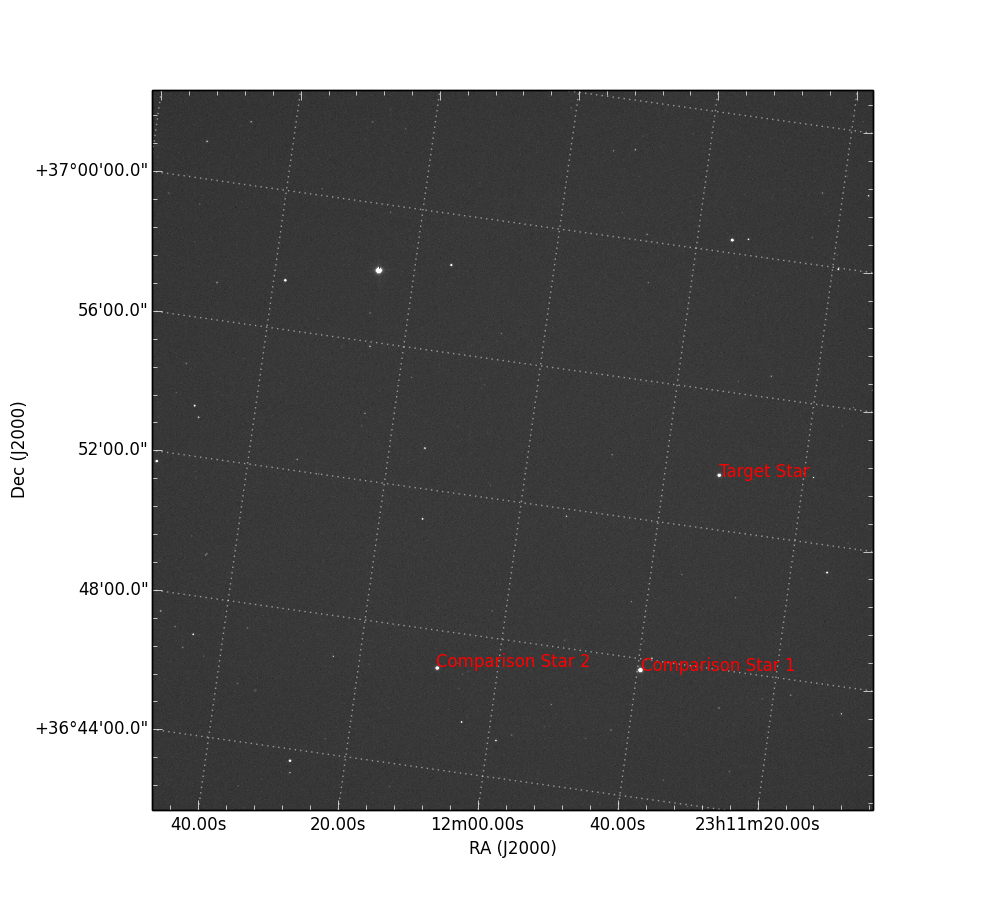
\includegraphics[scale=0.35]{StarMap}
\caption{\small{Mapping of Astrometry.net used to locate with RA and Dec. The target star shown with two comparison stars before the telescope passed into its hard limit. }}
\end{figure}
\end{center}

\begin{center}
\begin{figure}
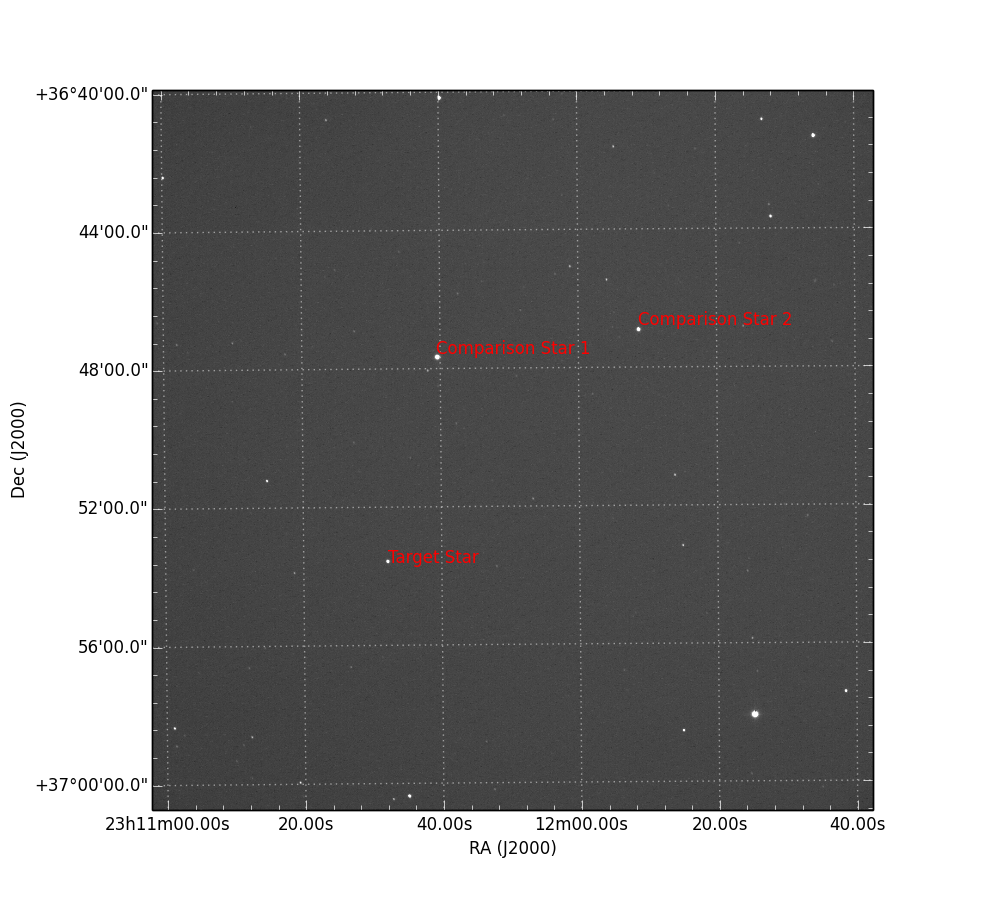
\includegraphics[scale= 0.35]{StarMap2}
\caption{\small{Mapping of Astrometry.net used to locate with RA and Dec. The target star shown with two comparison stars after the telescope emerged out of its hard limit, and image taking resumed.}}
\end{figure}
\end{center}

\begin{center}
\begin{figure}
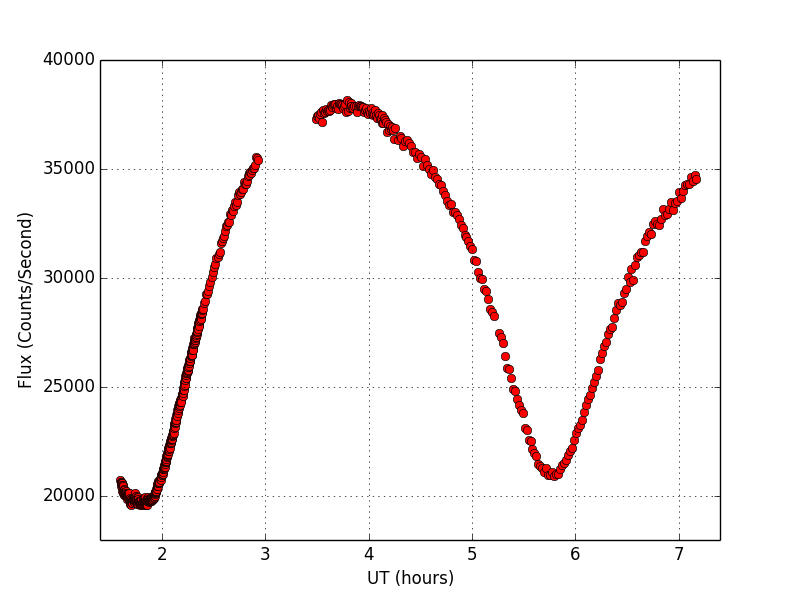
\includegraphics[scale=0.35]{detrend_1}
\caption{\small{Flux of the binary stars AB And over the duration of both primary and secondary eclipses. Flux on the y-axis and UT time in hours on the x-axis}}
\end{figure}
\end{center}

\begin{center}
Table 1
\end{center}
\begin{center}
\begin{tabular}{|l|l|}
\hline
\multicolumn{2}{|c|}{AB And} \\
\hline
Star 1 $T_{eff}$  & 5670 K  \\
Star 2 $T_{eff}$  & 5370 K  \\
Period & 7.965432 hours \\
Inclination & 87.3 \\
Eccentricity & 0.0 \\
Mass Ratio & 0.75 \\
\hline
\end{tabular}
\end{center}







\begin{center}
\begin{figure}
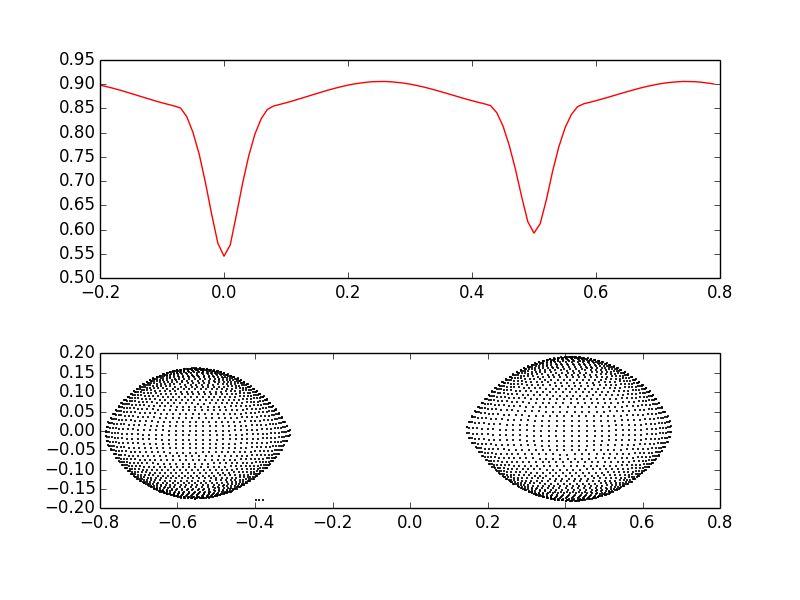
\includegraphics[scale=0.25]{figure_2}
\caption{\small{Using parameters determined by previous researchers to acquire an appropriate light curve for the binary star system AB And. This graph will be used as the control to compare the other graphs to.}}
\end{figure}
\end{center}

\begin{center}
\begin{figure}
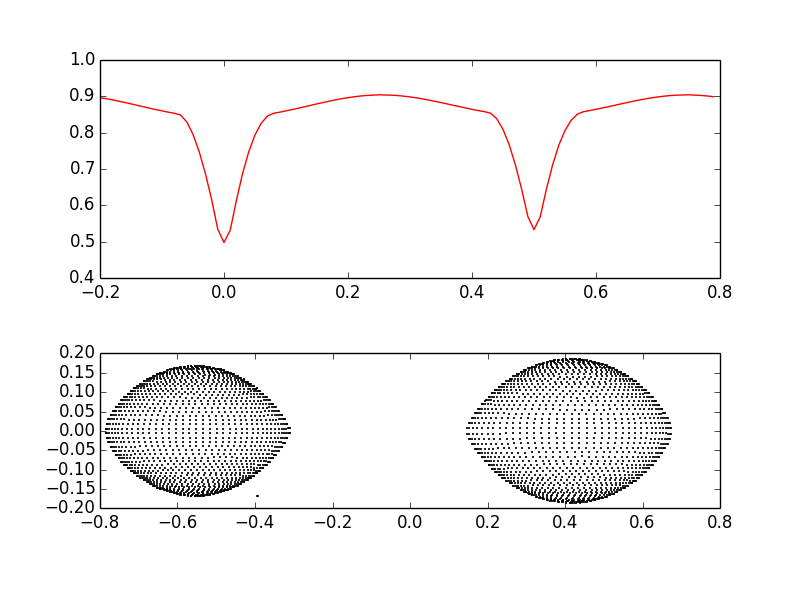
\includegraphics[scale=0.25]{figure_1}
\caption{\small{Shows an inclination of i = 90 (edge-on view), this is changed from i = 87.3. The drop in flux is much more difficult to tell there are two separate stars from the plot, but the total flux drop in each eclipse is different.}}
\end{figure}
\end{center}

\begin{center}
\begin{figure}
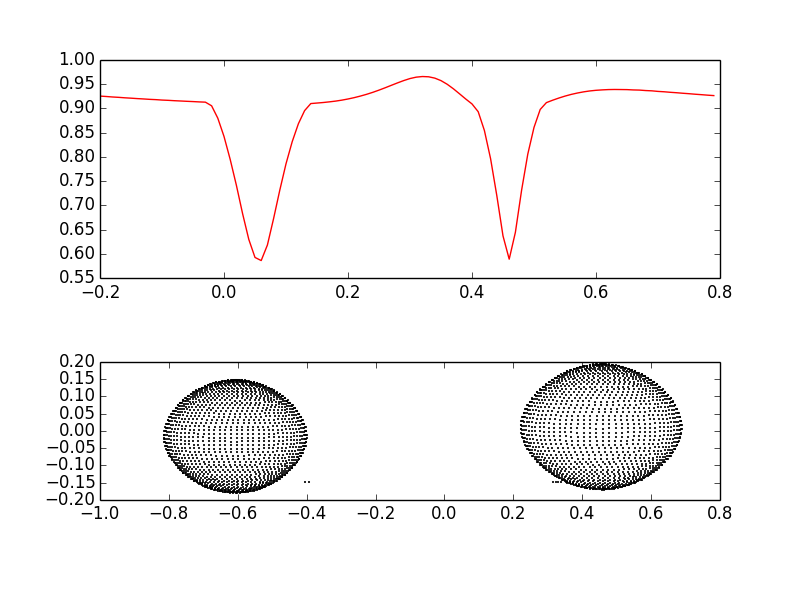
\includegraphics[scale=0.25]{figure_3}
\caption{\small{Shows how an increase in eccentricity in orbit affects the light curve, raising e from e =0.0 to e = 0.25. This causes and obvious bump in the light curve right before ingress begins.}}
\end{figure}
\end{center}

\begin{center}
\begin{figure}
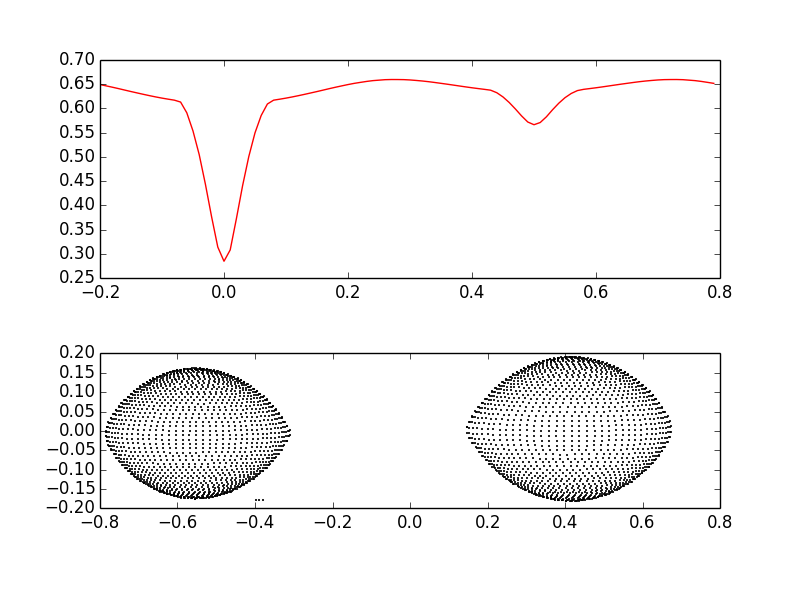
\includegraphics[scale=0.25]{figure_4}
\caption{\small{Shows how the difference in temperature can affect the depth of the flux drop during eclipse. The hotter star is increased in temperature by 3000 K.}}
\end{figure}
\end{center}

\begin{center}
\begin{figure}
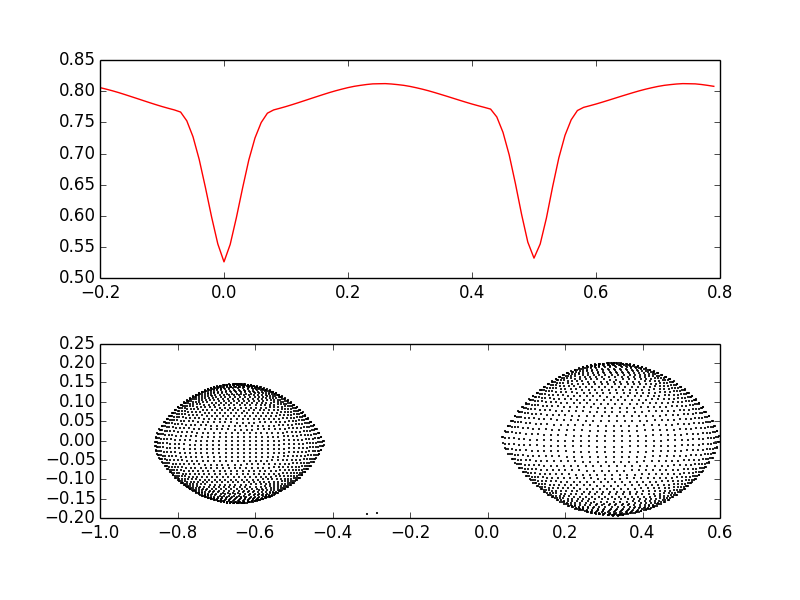
\includegraphics[scale=0.25]{figure_5}
\caption{\small{The Mass Ratio between the two star was changed so one star is twice the mass as the other. The depth of flux drop depends on temperature, not mass. Because the radii did not change, nothing in the light curve changes in comparison to the control.}}
\end{figure}
\end{center}

\begin{center}
\begin{figure}
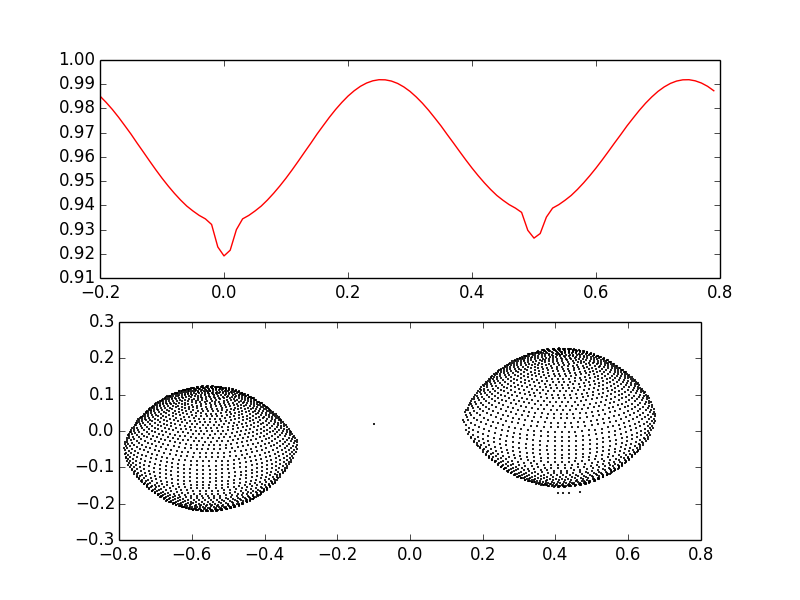
\includegraphics[scale=0.25]{figure_6}
\caption{\small{Here the inclination is changed to i = 70.0 making the eclipse almost impossible to see. Instead of the stars eclipsing over each other perfectly, they are now only overlapping on the edges. There is a strong curve still because the light from the Roche Lobes are still being blocked and exposed over and over. Only a small sudden drop is observed at the bottom of the valleys in the plot.}}
\end{figure}
\end{center}


\paragraph{Results}

\ \

From Plotting the data, many characteristics can be determined. From the two eclipse depths, it can be determined that the two stars have a relatively similar $T_{eff}$. The exact period cannot be determined from our plot but from the two dips, assuming low eccentricity of the orbits, the period is approximately 8 hours. Plotting our light curve against plots with different parameters, it can be seen that both Roche Lobes are being filled instead of both or a one of the two stars being spherical.

\paragraph{Conclusion}

\ \

Observing binary star systems can yield characteristics of both stars than cannot be determined by a single lone star. The light curve plotted doesn't show a second eclipse for both stars, so ideally more data would be taken. A second and third set of eclipses would be much greater than only a single set, so that the period could be determined with less uncertainty. Also taking spectroscopy of the two star would be ideal to calculate exact temperatures and more.

\ \

All binary systems are different in some manner, but viewing the light curve they produce can show incredibly fascinating characteristic of the system.

\end{document}



